% grains cheat sheet: two landscape A4 pages.  Build: make cheatsheet
% Every number here comes from lib/grains_ctl.h, lib/grains_voice.h,
% lib/grains.h and lib/grains_bank.h (dial values printed from that code).
\documentclass{article}
\usepackage[a4paper,landscape,margin=6mm]{geometry}
\usepackage[T1]{fontenc}
\usepackage{lmodern}
\usepackage[default]{sourcesanspro}
\usepackage{amssymb}
\usepackage{tikz}
\usepackage[most]{tcolorbox}
\usepackage{array}
\usepackage{tabularx}
\pagestyle{empty}
\setlength{\parindent}{0pt}

\definecolor{ink}{RGB}{30,30,30}
\definecolor{snd}{RGB}{20,20,20}       % SOUND-page knob labels
\definecolor{grc}{RGB}{0,130,120}      % GRAIN-page knob labels
\definecolor{fxc}{RGB}{30,90,170}      % FX-page knob labels
\definecolor{ampc}{RGB}{67,160,71}     % amp envelope
\definecolor{modc}{RGB}{230,140,20}    % mod envelope
\definecolor{lfoc}{RGB}{150,60,170}    % LFO
\definecolor{fltc}{RGB}{215,60,50}     % filter
\definecolor{freec}{RGB}{170,170,170}  % unassigned
\definecolor{padc}{RGB}{120,170,230}

\newcommand{\FX}[1]{\textcolor{fxc}{#1}}
\newcommand{\GR}[1]{\textcolor{grc}{#1}}
\newcommand{\cc}[1]{\textcolor{black!45}{\fontsize{4.6}{5}\selectfont #1}}

% knob: x, SOUND label (above), GRAIN label, FX label (below)
\newcommand{\knob}[4]{%
  \draw[fill=black!8, draw=black!60, line width=0.4pt] (#1,63) circle (3.4);
  \draw[black!60, line width=0.5pt] (#1,63) -- ++(110:2.9);
  \node[font=\fontsize{5.6}{6.2}\selectfont\bfseries, text=snd, align=center] at (#1,70.2) {#2};
  \node[font=\fontsize{5.4}{6}\selectfont\bfseries, text=grc, align=center] at (#1,56.4) {#3};
  \node[font=\fontsize{5.4}{6}\selectfont, text=fxc, align=center] at (#1,52.4) {#4};}
% pad: col (0..7), row (1 top, 0 bottom), label
\newcommand{\pad}[3]{%
  \draw[rounded corners=0.8mm, fill=padc!35!white, draw=padc!80!black, line width=0.4pt]
    (36+#1*13.2, 21+#2*13.2) rectangle ++(12,12);
  \node[font=\fontsize{5.4}{6}\selectfont, text=ink, align=center, text width=11mm]
    at (36+#1*13.2+6, 21+#2*13.2+6) {#3};}
% fader: x, top label, colour
\newcommand{\fader}[3]{%
  \draw[fill=black!12, draw=black!50] (#1-0.7,26) rectangle (#1+0.7,52);
  \draw[fill=#3!60!white, draw=#3!70!black, rounded corners=0.4mm] (#1-2.6,36) rectangle (#1+2.6,40);
  \node[font=\fontsize{5.6}{6.2}\selectfont\bfseries, text=#3!70!black, align=center] at (#1,56) {#2};}
% small button: x, y, label, colour, width
\newcommand{\btn}[5]{%
  \draw[rounded corners=0.6mm, fill=#4!25!white, draw=#4!70!black, line width=0.4pt]
    (#1-#5/2,#2-2.6) rectangle (#1+#5/2,#2+2.6);
  \node[font=\fontsize{4.9}{5.4}\selectfont, text=ink, align=center] at (#1,#2) {#3};}

\tcbset{card/.style={enhanced, colback=white, colframe=black!70, boxrule=0.5pt, arc=1.5mm,
    left=1.6mm, right=1.6mm, top=1.1mm, bottom=1.1mm, toptitle=0.6mm, bottomtitle=0.6mm,
    fonttitle=\bfseries\fontsize{8.6}{10}\selectfont, coltitle=white, colbacktitle=black!75,
    fontupper=\fontsize{7.1}{8.5}\selectfont, before skip=0mm, after skip=1.8mm}}
\newtcolorbox{card}[1]{card, title={#1}}
\newcolumntype{L}{>{\raggedright\arraybackslash}X}

\begin{document}

{\fontsize{16}{18}\selectfont\bfseries grains}\hspace{3mm}%
{\fontsize{9.5}{11}\selectfont Axoloti Core + Launchkey 49 MK3 (standalone mode) \textperiodcentered{}
mono granular synth, the SD-card patch \textperiodcentered{} \texttt{patches/grains/grains\_v1.axp}}\hfill
{\fontsize{7}{8}\selectfont\color{black!55} v1.0 \textperiodcentered{} 2026-11-05 \textperiodcentered{} page 1 of 2 \textperiodcentered{} github.com/ndlopes-github/axoloti-playground}

\vspace{1.5mm}
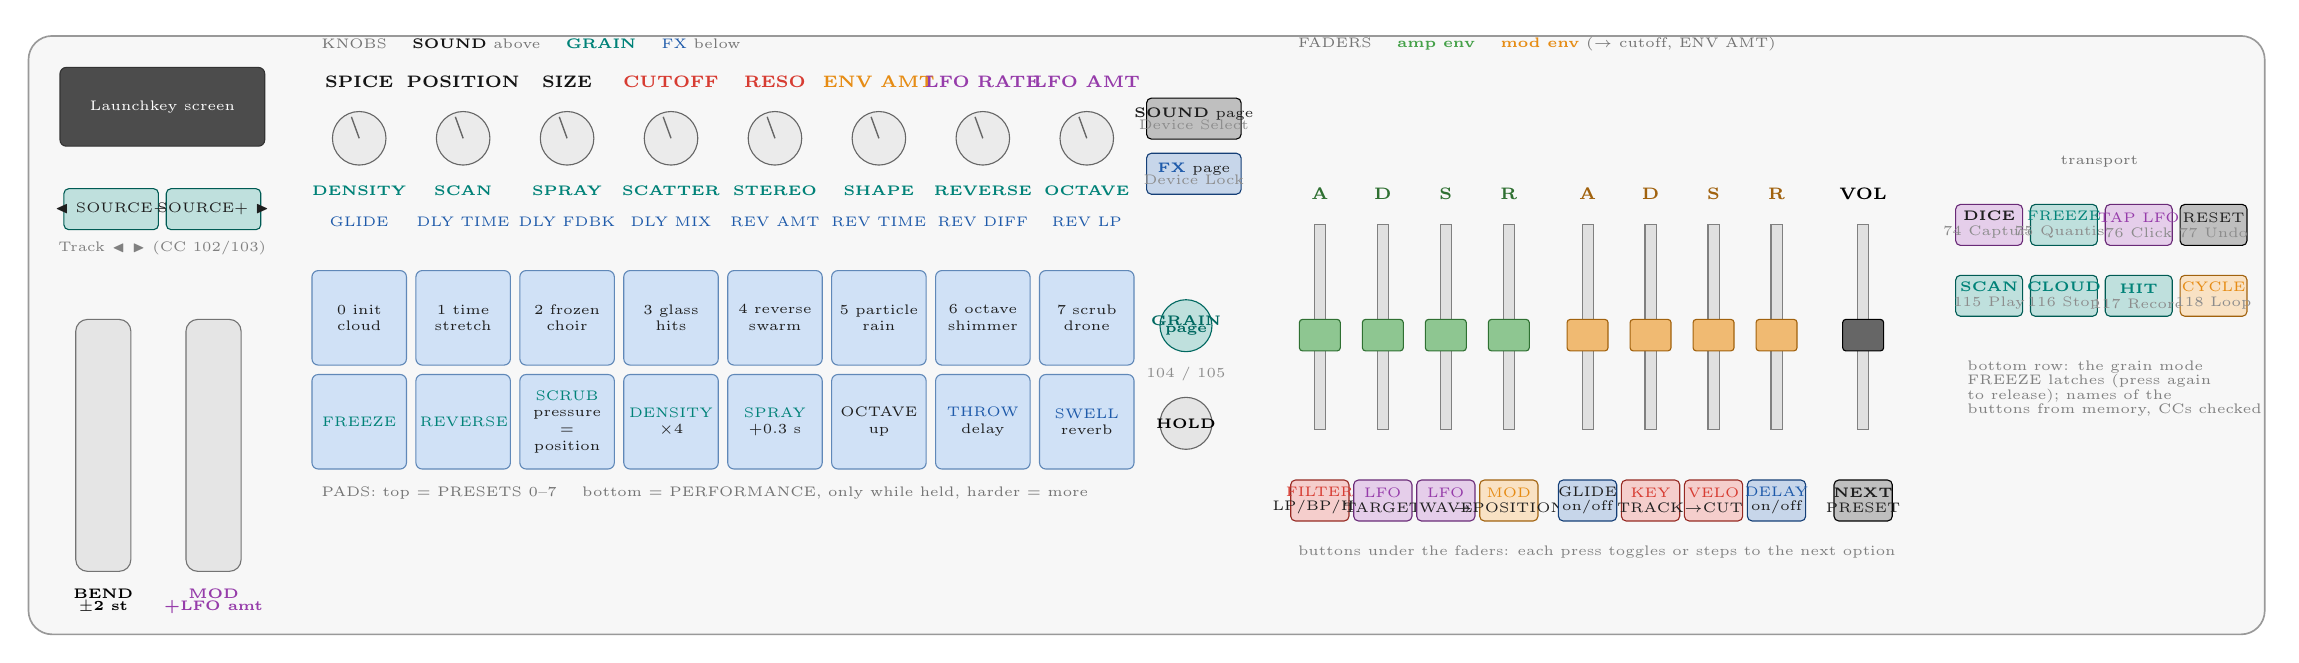
\begin{tikzpicture}[x=1mm,y=1mm]
  \draw[rounded corners=3mm, fill=black!3, draw=black!40, line width=0.6pt] (0,0) rectangle (284,76);

  % ---- left: screen, track buttons, wheels
  \draw[fill=black!70, draw=black!80, rounded corners=0.8mm] (4,62) rectangle (30,72);
  \node[font=\fontsize{5}{6}\selectfont, text=white] at (17,67) {Launchkey screen};
  \btn{10.5}{54}{\(\blacktriangleleft\) SOURCE\(-\)}{grc}{12}
  \btn{23.5}{54}{SOURCE+ \(\blacktriangleright\)}{grc}{12}
  \node[font=\fontsize{4.6}{5}\selectfont, text=black!50] at (17,49) {Track \(\blacktriangleleft\) \(\blacktriangleright\) (CC 102/103)};
  \draw[rounded corners=1.5mm, fill=black!10, draw=black!55] (6,8) rectangle (13,40);
  \draw[rounded corners=1.5mm, fill=black!10, draw=black!55] (20,8) rectangle (27,40);
  \node[font=\fontsize{5.4}{6}\selectfont\bfseries, align=center] at (9.5,4.2) {BEND\\[-0.6mm]\(\pm\)2 st};
  \node[font=\fontsize{5.4}{6}\selectfont\bfseries, align=center, text=lfoc] at (23.5,4.2) {MOD\\[-0.6mm]+LFO amt};

  % ---- knobs: SOUND (black, top) / GRAIN (green) / FX (blue)
  \node[font=\fontsize{5}{6}\selectfont, text=black!55, anchor=west] at (36,75) {KNOBS \quad
     \textbf{\textcolor{snd}{SOUND}} above \quad \textbf{\GR{GRAIN}} \quad \FX{FX} below};
  \knob{42}{SPICE}{\GR{DENSITY}}{\FX{GLIDE}}
  \knob{55.2}{POSITION}{\GR{SCAN}}{\FX{DLY TIME}}
  \knob{68.4}{SIZE}{\GR{SPRAY}}{\FX{DLY FDBK}}
  \knob{81.6}{\textcolor{fltc}{CUTOFF}}{\GR{SCATTER}}{\FX{DLY MIX}}
  \knob{94.8}{\textcolor{fltc}{RESO}}{\GR{STEREO}}{\FX{REV AMT}}
  \knob{108}{\textcolor{modc}{ENV AMT}}{\GR{SHAPE}}{\FX{REV TIME}}
  \knob{121.2}{\textcolor{lfoc}{LFO RATE}}{\GR{REVERSE}}{\FX{REV DIFF}}
  \knob{134.4}{\textcolor{lfoc}{LFO AMT}}{\GR{OCTAVE}}{\FX{REV LP}}
  \btn{148}{65.5}{\textbf{SOUND} page\\[-0.4mm]\cc{Device Select}}{black}{12}
  \btn{148}{58.5}{\textbf{\FX{FX}} page\\[-0.4mm]\cc{Device Lock}}{fxc}{12}

  % ---- pads + round buttons
  \pad{0}{1}{0 init\\cloud} \pad{1}{1}{1 time\\stretch} \pad{2}{1}{2 frozen\\choir} \pad{3}{1}{3 glass\\hits}
  \pad{4}{1}{4 reverse\\swarm} \pad{5}{1}{5 particle\\rain} \pad{6}{1}{6 octave\\shimmer} \pad{7}{1}{7 scrub\\drone}
  \pad{0}{0}{\GR{FREEZE}} \pad{1}{0}{\GR{REVERSE}} \pad{2}{0}{\GR{SCRUB}\\pressure\\= position} \pad{3}{0}{\GR{DENSITY}\\\(\times\)4}
  \pad{4}{0}{\GR{SPRAY}\\+0.3 s} \pad{5}{0}{OCTAVE\\up} \pad{6}{0}{\FX{THROW}\\delay} \pad{7}{0}{\FX{SWELL}\\reverb}
  \node[font=\fontsize{5}{6}\selectfont, text=black!55, anchor=west] at (36,18) {PADS: top = PRESETS 0--7 \quad bottom = PERFORMANCE, only while held, harder = more};
  \draw[fill=grc!25!white, draw=grc!80!black] (147,39.2) circle (3.3);
  \draw[fill=black!10, draw=black!60] (147,26.8) circle (3.3);
  \node[font=\fontsize{4.6}{5}\selectfont\bfseries, align=center, text=grc!80!black] at (147,39.2) {GRAIN\\[-0.8mm]page};
  \node[font=\fontsize{4.6}{5}\selectfont\bfseries, align=center] at (147,26.8) {HOLD};
  \node[font=\fontsize{4.2}{5}\selectfont, text=black!45] at (147,33) {104 / 105};

  % ---- faders
  \node[font=\fontsize{5}{6}\selectfont, text=black!55, anchor=west] at (160,75) {FADERS \quad
     \textcolor{ampc}{\textbf{amp env}} \quad \textcolor{modc}{\textbf{mod env}} (\(\to\) cutoff, ENV AMT)};
  \fader{164}{A}{ampc} \fader{172}{D}{ampc} \fader{180}{S}{ampc} \fader{188}{R}{ampc}
  \fader{198}{A}{modc} \fader{206}{D}{modc} \fader{214}{S}{modc} \fader{222}{R}{modc}
  \fader{233}{VOL}{black}
  \btn{164}{17}{\textcolor{fltc}{FILTER}\\LP/BP/HP}{fltc}{7.4}
  \btn{172}{17}{\textcolor{lfoc}{LFO}\\TARGET}{lfoc}{7.4}
  \btn{180}{17}{\textcolor{lfoc}{LFO}\\WAVE}{lfoc}{7.4}
  \btn{188}{17}{\textcolor{modc}{MOD}\\\(\to\)POSITION}{modc}{7.4}
  \btn{198}{17}{GLIDE\\on/off}{fxc}{7.4}
  \btn{206}{17}{\textcolor{fltc}{KEY}\\TRACK}{fltc}{7.4}
  \btn{214}{17}{\textcolor{fltc}{VELO}\\\(\to\)CUT}{fltc}{7.4}
  \btn{222}{17}{\FX{DELAY}\\on/off}{fxc}{7.4}
  \btn{233}{17}{\textbf{NEXT}\\PRESET}{black}{7.4}
  \node[font=\fontsize{4.6}{5}\selectfont, text=black!50, anchor=west] at (160,10.5) {buttons under the faders: each press toggles or steps to the next option};

  % ---- transport (ch 16)
  \node[font=\fontsize{5}{6}\selectfont, text=black!55] at (263,60) {transport};
  \btn{249}{52}{\textbf{DICE}\\\cc{74 Capture}}{lfoc}{8.5}
  \btn{258.5}{52}{\GR{FREEZE}\\\cc{75 Quantise}}{grc}{8.5}
  \btn{268}{52}{\textcolor{lfoc}{TAP LFO}\\\cc{76 Click}}{lfoc}{8.5}
  \btn{277.5}{52}{RESET\\\cc{77 Undo}}{black}{8.5}
  \btn{249}{43}{\GR{\textbf{SCAN}}\\\cc{115 Play}}{grc}{8.5}
  \btn{258.5}{43}{\GR{\textbf{CLOUD}}\\\cc{116 Stop}}{grc}{8.5}
  \btn{268}{43}{\GR{\textbf{HIT}}\\\cc{117 Record}}{grc}{8.5}
  \btn{277.5}{43}{\textcolor{modc}{CYCLE}\\\cc{118 Loop}}{modc}{8.5}
  \node[font=\fontsize{4.6}{5.2}\selectfont, text=black!50, align=left, anchor=north west] at (245,36)
     {bottom row: the grain mode\\FREEZE latches (press again\\to release); names of the\\buttons from memory, CCs checked};
\end{tikzpicture}

\vspace{1.2mm}
\begin{minipage}[t]{76mm}\vspace{0pt}
\begin{card}{Knobs: three pages, scaled pickup}
\fontsize{6.8}{8.1}\selectfont
\begin{tabularx}{\linewidth}{@{}l L@{}}
\textbf{SPICE} & chaos: each phrase gets its own position (\(\pm\)0.25), pitch (\(\pm\)0.5 st) and cutoff (\(\pm\)1.5 oct)
offset, and all grains more spray (+0.1 s), scatter (+3 st), reversal (+0.3) and width (+0.5) \\
\textbf{POSITION} & where in the source, 0 -- 1 (SCAN: where a phrase starts) \\
\textbf{SIZE} & grain length 5 ms -- 1 s (exponential) \\
\textbf{knobs 4--8} & \textcolor{fltc}{CUTOFF}, \textcolor{fltc}{RESO}, \textcolor{modc}{ENV AMT}, \textcolor{lfoc}{LFO RATE}, \textcolor{lfoc}{LFO AMT}: as freak \\[0.5mm]
\GR{\textbf{DENSITY}} & 0.5 -- 200 grains/s; in HIT, grains per note, 1 -- 20 \\
\GR{\textbf{SCAN}} & SCAN speed: centre = still, right forward, left backward, \(\frac1{16}\) -- 4\(\times\) \\
\GR{\textbf{SPRAY}} & random start, \(\pm\)0 -- 0.5 s \\
\GR{\textbf{SCATTER}} & random pitch, \(\pm\)0 -- 12 st \\
\GR{\textbf{STEREO}} & random pan width, 0 -- 1 \\
\GR{\textbf{SHAPE}} & grain window: smooth (bell) \(\to\) percussive (4\,\% attack) \\
\GR{\textbf{REVERSE}} & chance a grain plays backwards \\
\GR{\textbf{OCTAVE}} & chance a grain jumps an octave, up or down \\[0.5mm]
\FX{FX page} & as freak: GLIDE; delay (now stereo); reverb \\
\end{tabularx}
\vspace{0.4mm}
\textbf{Pages}: Device Select = SOUND, round button (upper, right of the pads) = \GR{GRAIN}, Device Lock = FX.
A knob left behind by a page change, preset or DICE moves the value proportionally until they meet: no jumps.
\end{card}
\end{minipage}\hfill
\begin{minipage}[t]{68mm}\vspace{0pt}
\begin{card}{Grain modes (Play / Stop / Record)}
\GR{\textbf{SCAN}}: grains at a steady rate from a play head that moves through the source at SCAN speed,
from POSITION on each new phrase: time stretch, slow motion, reverse, still.\\[0.4mm]
\GR{\textbf{CLOUD}}: grains at random times (mean = DENSITY) around POSITION: textures.\\[0.4mm]
\GR{\textbf{HIT}}: each note fires DENSITY grains at once, then nothing: percussive. Short SHAPE and a
plucky amp envelope suit it.\\[0.4mm]
C4 (middle C) plays a source at its own pitch; keys transpose the grains (\(-\)48 to +36 st).
\end{card}
\begin{card}{Keys: mono, legato, hold}
The newest key sounds; release it and the previous one comes back, without restarting (legato).
A key with no other down starts a \emph{phrase}: envelopes restart, SCAN jumps to POSITION,
SPICE rolls. GLIDE as freak. \textbf{HOLD} (round button, lower) or the sustain pedal keeps the note
after release; a new key then starts a new phrase.
\end{card}
\begin{card}{Envelopes, filter, LFO}
As freak: faders 1--4 amp, 5--8 mod (1 ms -- 10 s; S 0 -- 1); CYCLE (Loop) loops the mod env.
Mod env \(\to\) cutoff (ENV AMT) and \(\to\) position (+0.5) with MOD\(\to\)POSITION. Grains keep coming
while the amp envelope is open, release included.
Filter: stereo 12 dB/oct SVF, LP/BP/HP. LFO TARGET: \textbf{position} (\(\pm\)0.5) \(\to\) size (\(\times\frac14\)--4)
\(\to\) cutoff (\(\pm\)3 oct) \(\to\) pitch (\(\pm\)2 st); WAVE and TAP as freak.
\end{card}
\end{minipage}\hfill
\begin{minipage}[t]{66mm}\vspace{0pt}
\begin{card}{Sources}
\textbf{SOURCE} (Track \(\blacktriangleleft\)\,/\,\(\blacktriangleright\)) steps through what is loaded: 0 = built-in
(a saw chord that brightens along its 1.5 s), 1--8 = the starter bank (page 2), then your files.
Presets name a source; one that is not loaded plays the built-in one.\\[0.4mm]
\textbf{Your own}: WAV files in \texttt{/grains} on the SD card, up to 16, loaded in name order
(name them \texttt{09\_xxx.wav}, at most 8 characters before \texttt{.wav}). 16, 24 or 32-bit or float;
any rate; stereo is mixed to mono. Memory: 7.2 MB in all, 3 MB of it the starter bank, so about
45 s at 48 kHz for your own (the log shows what is left).
Put them there with \emph{Board \(\to\) Enter Card Reader Mode}.\\[0.4mm]
Loading runs in the background after power-up (the starter bank: 1.1 s): until a source is
there, the built-in one plays.
\end{card}
\begin{card}{Pads}
\textbf{Top} = presets 0--7. \textbf{Bottom} = performance, while held; strike velocity, then
pressure, sets the amount:
\fontsize{6.6}{7.9}\selectfont
\begin{tabularx}{\linewidth}{@{}l L@{}}
\GR{FREEZE} & the position stops (SCAN head too) \\
\GR{REVERSE} & grains backwards, SCAN runs backwards \\
\GR{SCRUB} & pad pressure \emph{is} the position \\
\GR{DENSITY / SPRAY} & up to 4\(\times\) / +0.3 s \\
OCTAVE & +12 st \\
\FX{THROW / SWELL} & delay throw / reverb swell, as freak \\
\end{tabularx}
\end{card}
\end{minipage}\hfill
\begin{minipage}[t]{57mm}\vspace{0pt}
\begin{card}{Two patches, one board}
\textbf{SD card in} at power-up: grains starts. \textbf{No card}: freak (in flash) starts.\\[0.4mm]
\textbf{Install}: open \texttt{grains\_v1.axp}, \emph{Upload to SD Card as Startup}. That also copies the
starter bank to \texttt{/grains} (and replaces an older startup patch on the card).\\[0.4mm]
\textbf{If grains will not start}: power off, take the card out: freak starts. Then see page 2.
\end{card}
\begin{card}{Signal path and load}
20 grains (pool) \(\to\) stereo SVF \(\to\) amp env \(\times\) velocity \(\to\) stereo delay
\(\to\) Elements reverb \(\to\) VOL. When the pool is full, new grains wait: the load stays bounded.
DSP 41\,\% idle, 75.5\,\% with all 20 grains; patch RAM 28 of 44 KB.
\end{card}
\begin{card}{Notes}
Toggle states are not shown (no LEDs in standalone mode). With the patcher connected, its log reports the
loaded files, pages, presets, modes, sources and knobs catching up.
\end{card}
\end{minipage}

%======================================================================
\newpage
{\fontsize{16}{18}\selectfont\bfseries grains}\hspace{3mm}%
{\fontsize{9.5}{11}\selectfont starter bank, presets, dial values, troubleshooting}\hfill
{\fontsize{7}{8}\selectfont\color{black!55} v1.0 \textperiodcentered{} page 2 of 2}

\vspace{1.5mm}
\begin{minipage}[t]{166mm}\vspace{0pt}
\begin{card}{Starter bank: \texttt{/grains/01..08.wav}, 4 s each, made with freak's oscillators at C4 \quad\textmd{\fontsize{6.5}{7}\selectfont (each changes along its length, so POSITION matters)}}
\fontsize{7.2}{8.7}\selectfont
\begin{tabularx}{\linewidth}{@{}>{\bfseries}l L >{\bfseries}l L@{}}
1 & vowel FOF on C and G: a \(\to\) e \(\to\) i \(\to\) o \(\to\) u along the source &
5 & particles, density and pitch spread rising \\
2 & paraphonic chords, a new chord each second &
6 & feedback FM, more modulation along it, a new ratio each second \\
3 & harmonics, their centre rising (dark \(\to\) bright) &
7 & plucked arpeggio C E G B D B G E, 8 notes a second \\
4 & bell, 8 strikes (one per 0.5 s), more inharmonic each time &
8 & saw swarm C3 G3 C4, detune rising, filter opening \\
\end{tabularx}
\end{card}

\begin{card}{Presets: top pads = 0--7; NEXT PRESET (fader button 9) steps; RESET (Undo) = 0 \quad\textmd{\fontsize{6.5}{7}\selectfont (chosen from the parameter meanings, not yet tuned by ear)}}
\fontsize{7.2}{8.7}\selectfont
\begin{tabularx}{\linewidth}{@{}>{\bfseries}l L@{}}
0 init cloud & CLOUD on source 1 (vowels), middle; 140 ms grains, 22/s, half width; LP 4.7 kHz; delay off. The power-on sound. \\
1 time stretch & SCAN source 2 (chords) from the start at half speed: every chord lasts twice as long, pitch unchanged. \\
2 frozen choir & SCAN still, source 1 at 0.43: 320 ms grains, 44/s, wide, some octaves; slow triangle LFO drifts the
position; attack 0.33 s, release 3 s. Hold a note. \\
3 glass hits & HIT on source 4 (bells) at a strike: 11 percussive grains per note, wide, some octaves; decay 0.7 s. Play rhythms. \\
4 reverse swarm & CLOUD on source 8 (saw swarm): 87\,\% of the grains backwards, S\&H LFO on grain size. \\
5 particle rain & CLOUD on source 5 (particles): 40 ms grains at 90/s, spray 0.25 s, \(\pm\)2.7 st, full width,
percussive; S\&H LFO on cutoff. \\
6 octave shimmer & CLOUD on source 3 (harmonics): long grains, 80\,\% jump an octave; attack 0.7 s, release 3 s; big reverb. \\
7 scrub drone & SCAN source 7 (plucks) at 0.07\(\times\): a frozen arpeggio slowly turning; CYCLE on; glide. \\
\end{tabularx}\\[0.3mm]
A preset sets the mode, the source, all three knob pages, faders 1--8 and the toggles; the volume stays.
\textbf{DICE} (Capture MIDI) rolls the mode and the SOUND and GRAIN pages instead; source, envelopes, FX and volume stay.
\end{card}

\begin{card}{Sound design moves}
\fontsize{7.4}{9.0}\selectfont
\textbf{Time freeze}: SCAN with SCAN at the centre, or hold FREEZE; then sweep POSITION by hand or SCRUB with pressure.\quad
\textbf{Texture from anything}: CLOUD, SIZE 1/2, DENSITY 3/4, SPRAY 1/4, STEREO full.\quad
\textbf{Glitch}: HIT, SIZE 1/4, SHAPE full, SCATTER 1/2, play fast.\quad
\textbf{Moving drone}: LFO TARGET position, slow triangle, MOD\(\to\)POSITION with CYCLE on.\quad
\textbf{Pitched clouds}: SCATTER 0, OCTAVE 1/2, the Launchkey's Scale mode.
\end{card}
\end{minipage}\hfill
\begin{minipage}[t]{112mm}\vspace{0pt}
\begin{card}{Where the values fall (knob turned \dots)}
\fontsize{7.5}{9.2}\selectfont
\setlength{\tabcolsep}{3pt}
\begin{tabular}{@{}l r r r r@{}}
 & 1/4 & 1/2 & 3/4 & full \\ \hline
\textbf{SIZE} & 19 ms & 72 ms & 0.26 s & 1 s \\
\GR{\textbf{DENSITY}} (grains/s) & 2.3 & 10 & 44 & 200 \\
\GR{\textbf{DENSITY}} in HIT (grains/note) & 6 & 11 & 15 & 20 \\
\GR{\textbf{SCAN}} (\(\times\) real time) & \(-\)0.45 & still & +0.42 & +4 \\
\GR{\textbf{SPRAY}} (\(\pm\)) & 32 ms & 0.13 s & 0.28 s & 0.5 s \\
\GR{\textbf{SCATTER}} (\(\pm\)) & 0.8 st & 3 st & 6.7 st & 12 st \\
\end{tabular}\\[0.5mm]
SCAN: still from 61 to 67 (the centre); \(\times\)1 at about 5/6 of the travel (and \(-\)1 at 1/6).
Envelopes, CUTOFF, RESO, ENV AMT, LFO, GLIDE, delay and VOL fall as on the freak card.
\end{card}

\begin{card}{Something seems wrong?}
\fontsize{7.5}{9.2}\selectfont
\textbf{No sound}: VOL up? In HIT, sound only comes on a key press. SIZE and DENSITY not both at the bottom?
CUTOFF as on freak.\\[0.4mm]
\textbf{Only the built-in sound}: no \texttt{/grains} folder, or the files are still loading or not WAV
(the log says which). Upload the patch to the SD card again to copy the bank.\\[0.4mm]
\textbf{Sound stuck on}: HOLD or the sustain pedal. Press HOLD (round button, lower).\\[0.4mm]
\textbf{Nothing moves}: FREEZE latched (Quantise), or SCAN at its centre.\\[0.4mm]
\textbf{grains does not start, or hangs}: power off, remove the card, power on: freak starts from flash.
Fix the card with Card Reader Mode (rename \texttt{/start.bin} to skip grains).\\[0.4mm]
\textbf{Lost}: RESET (Undo).
\end{card}

\begin{card}{MIDI reference (beyond the freak card)}
\fontsize{7.4}{9.0}\selectfont
\setlength{\tabcolsep}{3pt}
\begin{tabular}{@{}l l@{}}
GRAIN page / HOLD (round buttons) & ch 16 CC 104 / 105 \\
SCAN, CLOUD, HIT (Play, Stop, Record) & ch 16 CC 115, 116, 117 \\
FREEZE latch (Quantise) & ch 16 CC 75 \\
SOURCE \(-\) / + (track \(\blacktriangleleft\)/\(\blacktriangleright\)) & ch 16 CC 102 / 103 \\
sustain pedal (= HOLD while down) & ch 1 CC 64 \\
\end{tabular}
\end{card}
\end{minipage}

\end{document}
